% The reference page, de-warped, with its stems traced. Page 1 is the photo
% with the fitted page plane; page 2 is the rectified photo at 0.456 pt per
% pixel (the page's own scale) with the traced splines on top; page 3 sets
% the rectified photo beside the first demo page (build/demo.pdf, from
% `just build demo`) at the same scale, tops aligned.
\documentclass[tikz,border=0pt]{standalone}
\usepackage{graphicx}
\directlua{flora_ref = dofile("tex/reference/overlay.lua")}
\begin{document}
\begin{tikzpicture}
  \directlua{flora_ref.photo("analysis/source/reference-photo.png", 1109, 1568, 0.51)}
\end{tikzpicture}
\begin{tikzpicture}
  \directlua{flora_ref.rectified("tex/reference/rectified.png")}
\end{tikzpicture}
\IfFileExists{build/demo.pdf}{%
\begin{tikzpicture}
  \node[anchor=north west,inner sep=0] (ref) at (0,0)
    {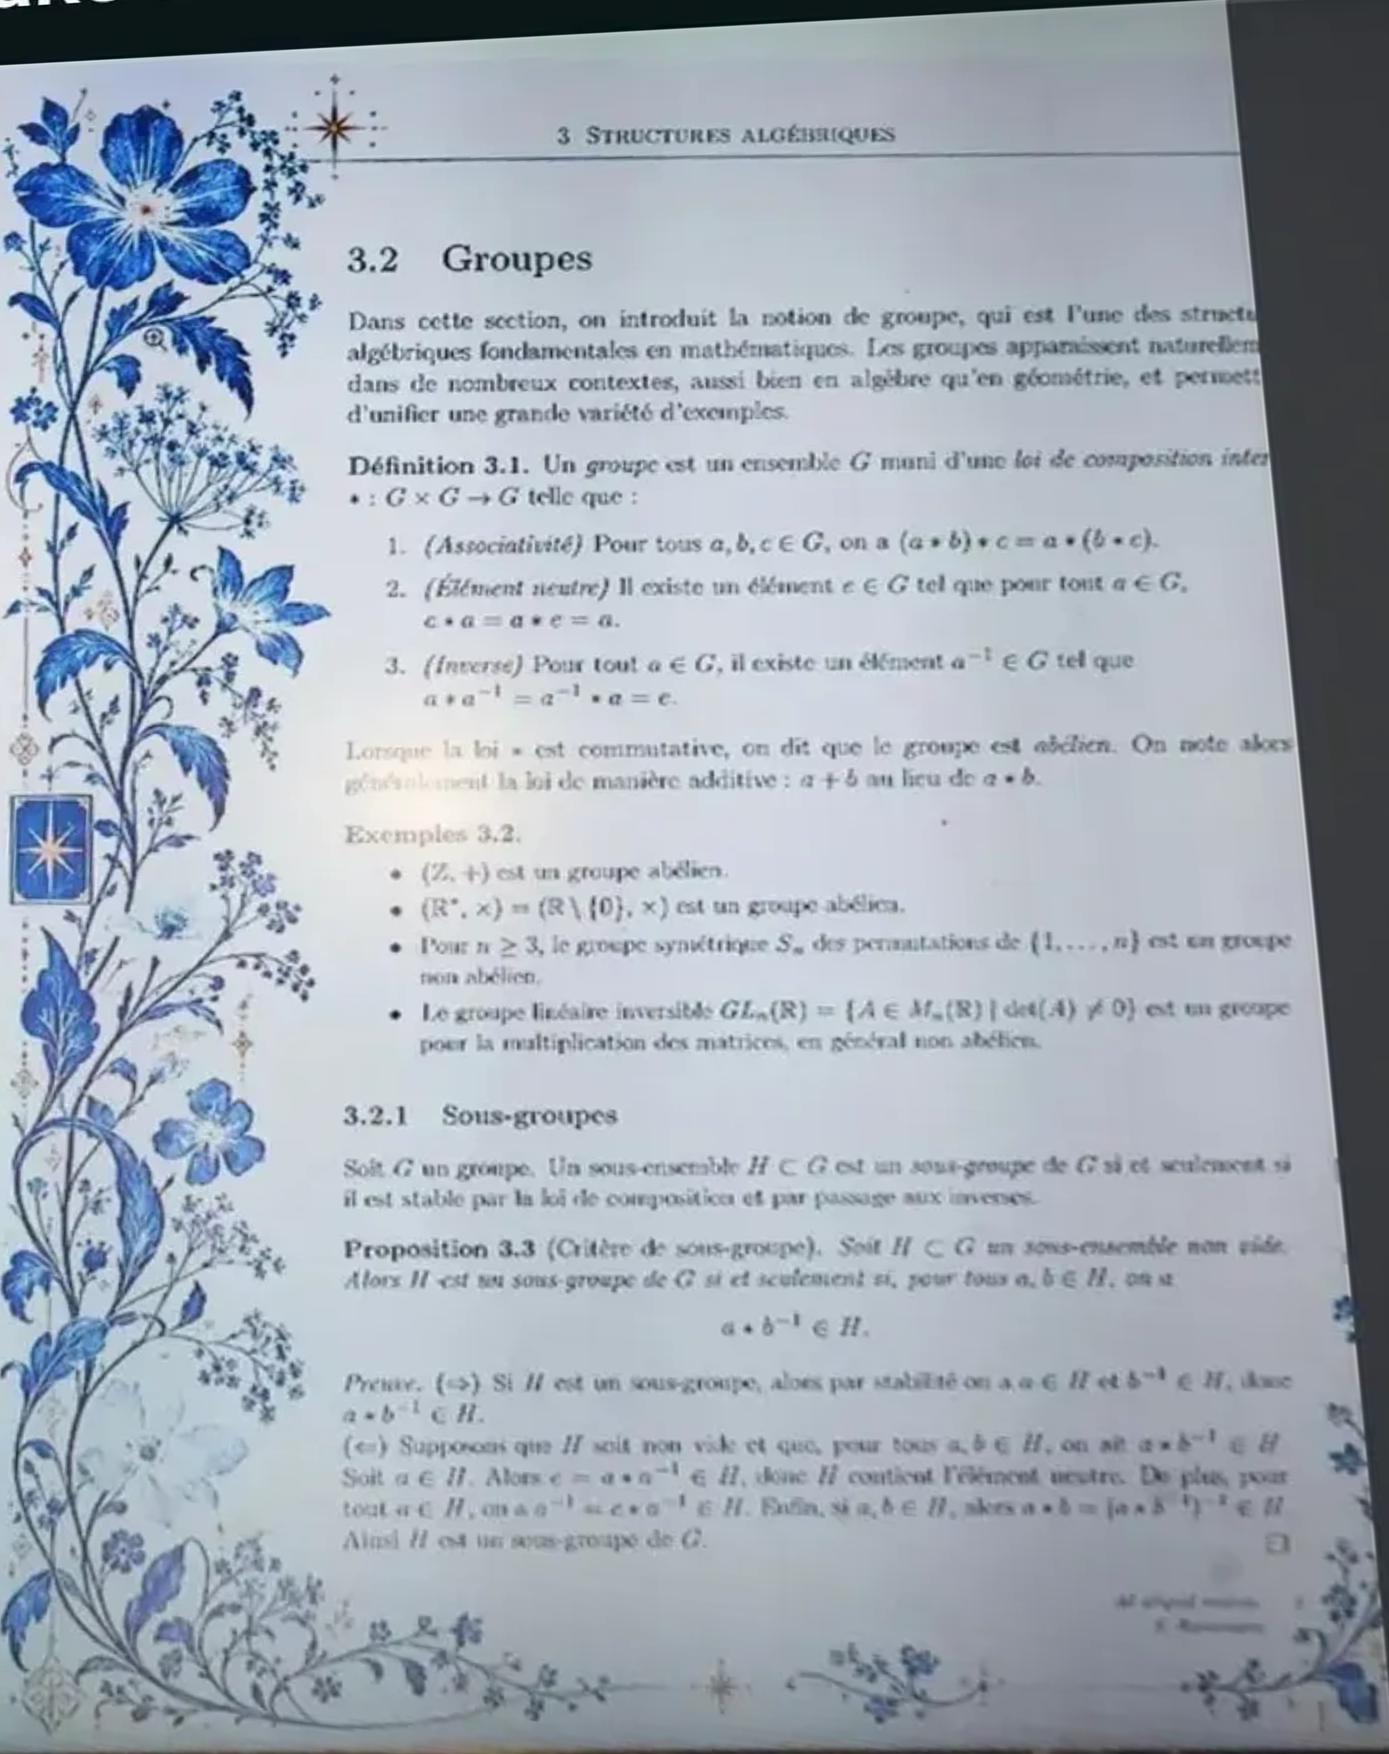
\includegraphics[width=\directlua{tex.print(flora_ref.width_pt())}pt]{tex/reference/rectified.png}};
  \node[anchor=north west,inner sep=0] at ([xshift=12pt]ref.north east)
    {\includegraphics[page=1]{build/demo.pdf}};
\end{tikzpicture}}{}
\end{document}
